	\large \bf{\textsc{\section{Lab 1}}
	\begin{problem}
		Choose a 15K\(\Omega\) resistor. Read the color code and tolerance.
		\newline
		1. Measure the resistance using a multimeter.
		\newline
		2. Adjust the power supply on 5V. Connect the resistors to the power supply. Measure the voltage and the current of the resistor.
		\newline
		3. Repeat step two for 11 different voltages ranging from -15V to 15V.
		\newline
		4. Plot the I-V characteristics of the resistors. Are all measurements on one line? What is the slope of the line? Compare it with your readings of the code and tolerance as well as the multimeter readings. 
	\end{problem}

	\begin{solution}
		1.
		\newline
		2.
		\newline
		3. 
		\begin{table}[h]
			\begin{tabular}{| l | l | l | l | l | l | l | l | l | l | l | l |}
				\hline
				\textbf{Try} & 1 & 2 & 3 & 4 & 5 & 6 & 7 & 8 & 9 & 10 & 11 \\ \hline
				Voltage (V)  & & & & & & & & & & & \\ \hline
				Current (mA) & & & & & & & & & & & \\ \hline
			\end{tabular}
		\end{table}
		\newline
		4.
	\end{solution}
	
	\begin{problem}
		Choose the following resistors and construct each circuit given in the figure. \\
		R\(_{1}\): 15K\(\Omega\) \\
		R\(_{2}\): 22K\(\Omega\) \\
		R\(_{3}\): 33K\(\Omega\) \\
		R\(_{4}\): 10K\(\Omega\) \\
		\newline
		1. Calculate the equivalent resistance.
		\newline
		2. Measure the resistance of each indicated terminal using multimeter.
		\newline
		3. Are they different? Check out the tolerances and conclude why there is a difference.
		\begin{figure}[h!]
			\centering
			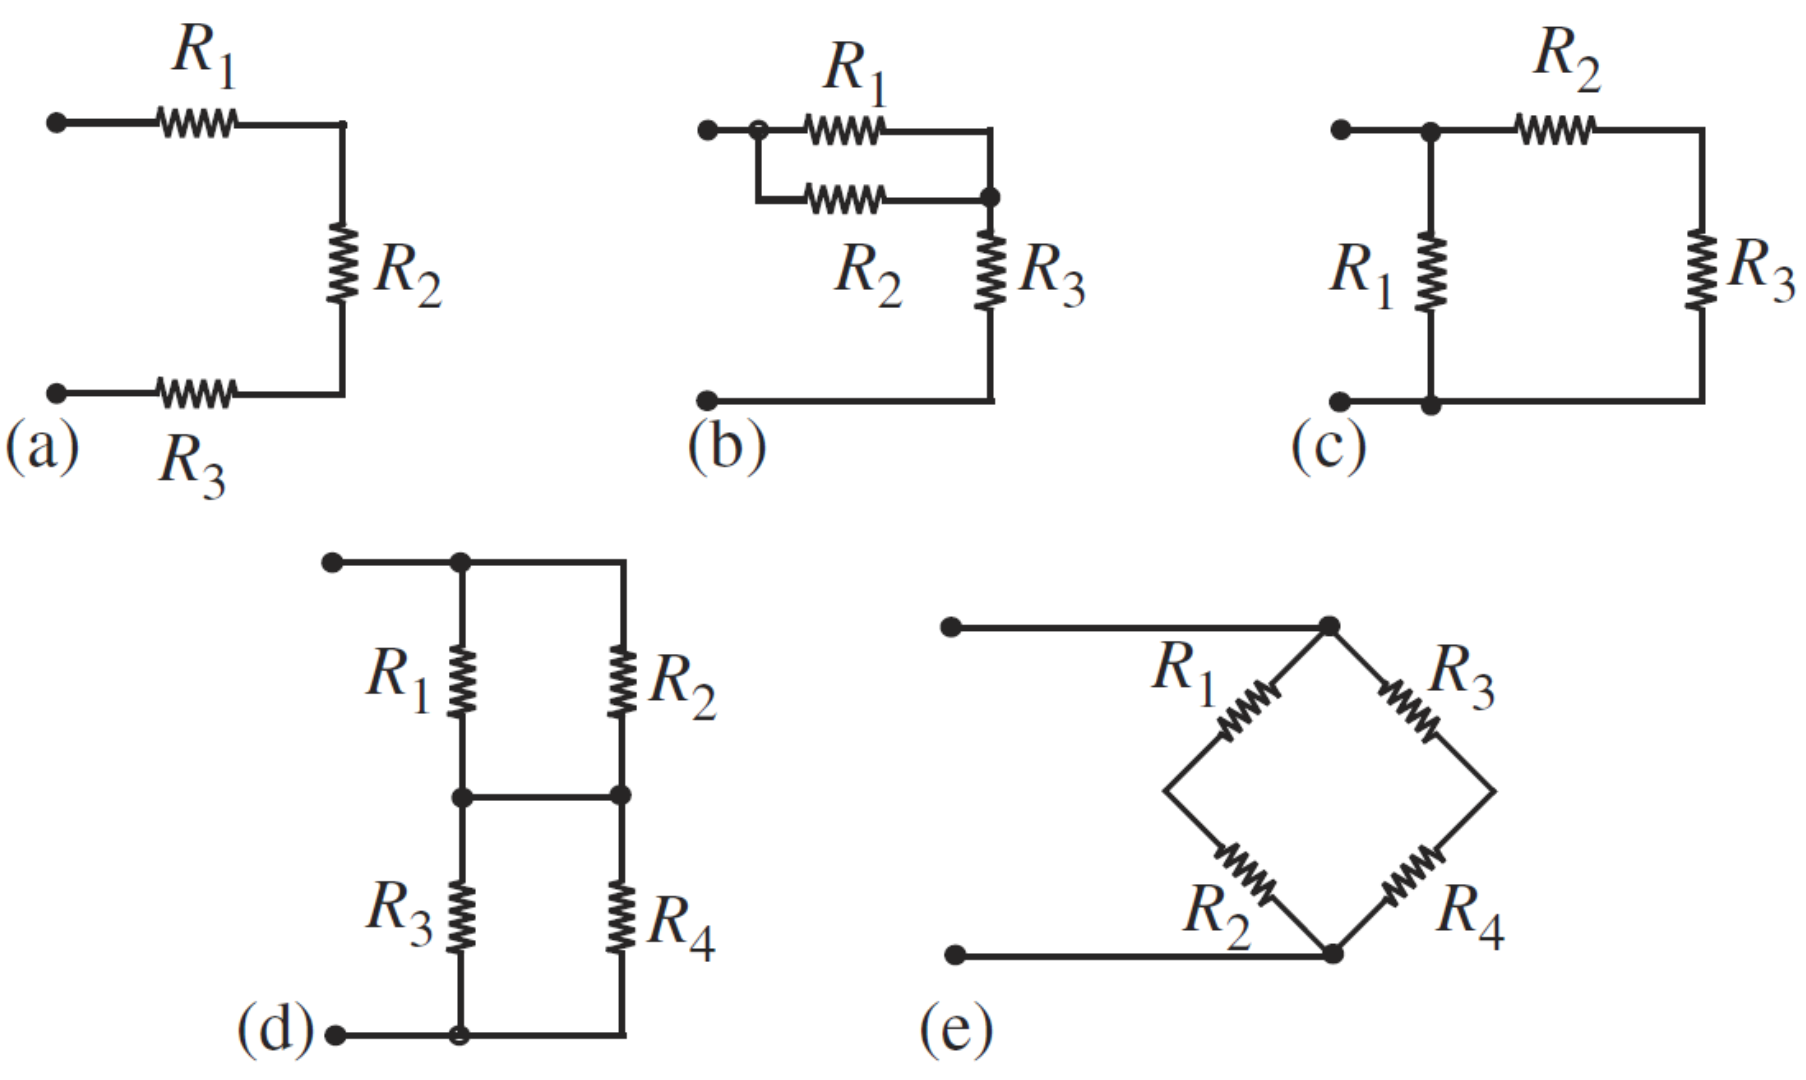
\includegraphics[width=0.5\textwidth]{images/figure1.png}
		\end{figure}
	\end{problem}
	
	\begin{solution}
		1. 
		\newline
		2.
		\newline
		3. 
	\end{solution}
	
	\begin{problem}
		Construct the circuit given in the following figure.
		\newline
		V\(_{A}\): 5V \\
		V\(_{B}\): 10V \\
		R\(_{1}\): 22K\(\Omega\) \\
		R\(_{2}\): 33K\(\Omega\) \\
		R\(_{3}\): 10K\(\Omega\) \\
		\newline
		1. Find all voltages and currents using KVL and KCL method.
		\newline
		2. Measure all currents and voltages stated in the circuit.
		\newline
		3. Compare the results.
		\begin{figure}[h!]
			\centering
			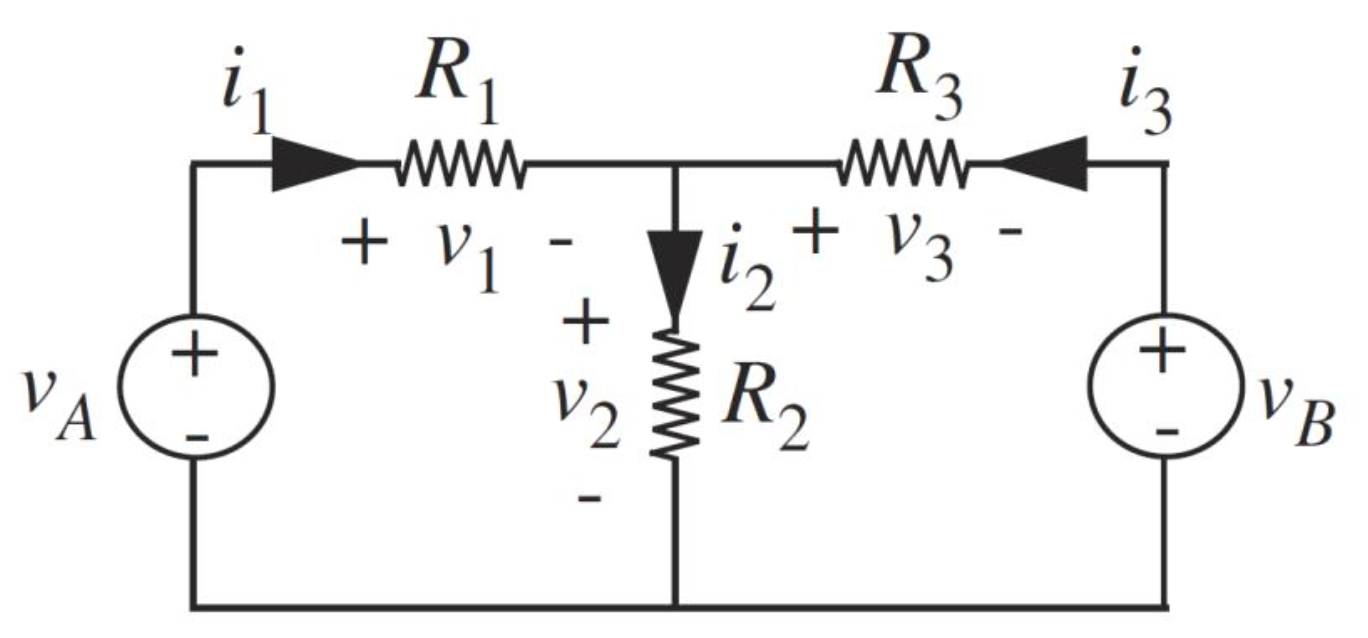
\includegraphics[width=0.5\textwidth]{images/circuit5.png}
		\end{figure}
	\end{problem}
	
	\begin{solution}
		1. 
		\newline
		2. 
		\newline
		3. 
	\end{solution}
		
	\begin{problem}
		Construct the circuit given in the following figure.
		\newline
		V\(_{A}\): 5V (with max current 60mA)\\
		I: 60mA (with max voltage 3V) \\
		R\(_{1}\): 180\(\Omega\) \\
		R\(_{2}\): 18\(\Omega\) \\
		R\(_{3}\): 270\(\Omega\) \\	
		\newline
		1. Calculate the voltage that falls on R\(_{3}\) using superposition.
		\newline
		2. Measure the voltage on R\(_{3}\).
		\newline
		3. Implement superposition in practice, by two tests (setting each source to zero and measuring the voltage)
		\newline
		4. Compare the results with your calculation.
		\newline
		5. Use the following resistors and explain why the measurements are not consistent with calculations\\
		R\(_{1}\): 180\(\Omega\) \\
		R\(_{2}\): 18\(\Omega\) \\
		R\(_{3}\): 270\(\Omega\) \\	
		\begin{figure}[h!]
			\centering
			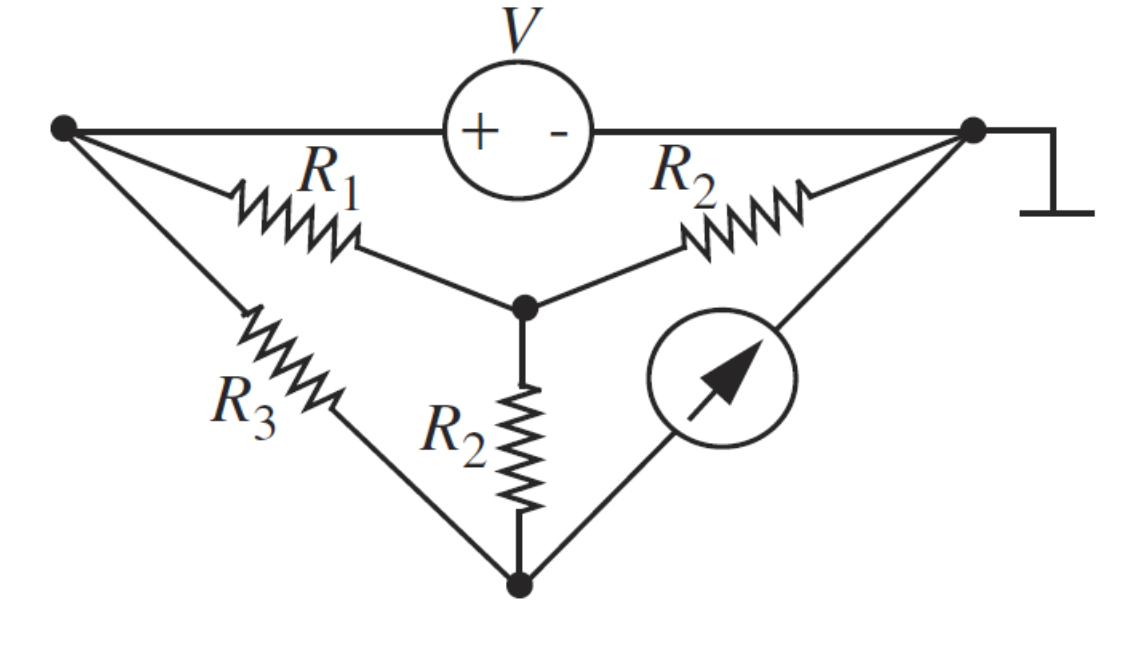
\includegraphics[width=0.5\textwidth]{images/circuit6.png}
		\end{figure}		
	\end{problem}
	
	\begin{solution}
		Solution goes here.
	\end{solution}